\documentclass[1p]{elsarticle_modified}
%\bibliographystyle{elsarticle-num}

%\usepackage[colorlinks]{hyperref}
%\usepackage{abbrmath_seonhwa} %\Abb, \Ascr, \Acal ,\Abf, \Afrak
\usepackage{amsfonts}
\usepackage{amssymb}
\usepackage{amsmath}
\usepackage{amsthm}
\usepackage{scalefnt}
\usepackage{amsbsy}
\usepackage{kotex}
\usepackage{caption}
\usepackage{subfig}
\usepackage{color}
\usepackage{graphicx}
\usepackage{xcolor} %% white, black, red, green, blue, cyan, magenta, yellow
\usepackage{float}
\usepackage{setspace}
\usepackage{hyperref}

\usepackage{tikz}
\usetikzlibrary{arrows}

\usepackage{multirow}
\usepackage{array} % fixed length table
\usepackage{hhline}

%%%%%%%%%%%%%%%%%%%%%
\makeatletter
\renewcommand*\env@matrix[1][\arraystretch]{%
	\edef\arraystretch{#1}%
	\hskip -\arraycolsep
	\let\@ifnextchar\new@ifnextchar
	\array{*\c@MaxMatrixCols c}}
\makeatother %https://tex.stackexchange.com/questions/14071/how-can-i-increase-the-line-spacing-in-a-matrix
%%%%%%%%%%%%%%%

\usepackage[normalem]{ulem}

\newcommand{\msout}[1]{\ifmmode\text{\sout{\ensuremath{#1}}}\else\sout{#1}\fi}
%SOURCE: \msout is \stkout macro in https://tex.stackexchange.com/questions/20609/strikeout-in-math-mode

\newcommand{\cancel}[1]{
	\ifmmode
	{\color{red}\msout{#1}}
	\else
	{\color{red}\sout{#1}}
	\fi
}

\newcommand{\add}[1]{
	{\color{blue}\uwave{#1}}
}

\newcommand{\replace}[2]{
	\ifmmode
	{\color{red}\msout{#1}}{\color{blue}\uwave{#2}}
	\else
	{\color{red}\sout{#1}}{\color{blue}\uwave{#2}}
	\fi
}

\newcommand{\Sol}{\mathcal{S}} %segment
\newcommand{\D}{D} %diagram
\newcommand{\A}{\mathcal{A}} %arc


%%%%%%%%%%%%%%%%%%%%%%%%%%%%%5 test

\def\sl{\operatorname{\textup{SL}}(2,\Cbb)}
\def\psl{\operatorname{\textup{PSL}}(2,\Cbb)}
\def\quan{\mkern 1mu \triangleright \mkern 1mu}

\theoremstyle{definition}
\newtheorem{thm}{Theorem}[section]
\newtheorem{prop}[thm]{Proposition}
\newtheorem{lem}[thm]{Lemma}
\newtheorem{ques}[thm]{Question}
\newtheorem{cor}[thm]{Corollary}
\newtheorem{defn}[thm]{Definition}
\newtheorem{exam}[thm]{Example}
\newtheorem{rmk}[thm]{Remark}
\newtheorem{alg}[thm]{Algorithm}

\newcommand{\I}{\sqrt{-1}}
\begin{document}

%\begin{frontmatter}
%
%\title{Boundary parabolic representations of knots up to 8 crossings}
%
%%% Group authors per affiliation:
%\author{Yunhi Cho} 
%\address{Department of Mathematics, University of Seoul, Seoul, Korea}
%\ead{yhcho@uos.ac.kr}
%
%
%\author{Seonhwa Kim} %\fnref{s_kim}}
%\address{Center for Geometry and Physics, Institute for Basic Science, Pohang, 37673, Korea}
%\ead{ryeona17@ibs.re.kr}
%
%\author{Hyuk Kim}
%\address{Department of Mathematical Sciences, Seoul National University, Seoul 08826, Korea}
%\ead{hyukkim@snu.ac.kr}
%
%\author{Seokbeom Yoon}
%\address{Department of Mathematical Sciences, Seoul National University, Seoul, 08826,  Korea}
%\ead{sbyoon15@snu.ac.kr}
%
%\begin{abstract}
%We find all boundary parabolic representation of knots up to 8 crossings.
%
%\end{abstract}
%\begin{keyword}
%    \MSC[2010] 57M25 
%\end{keyword}
%
%\end{frontmatter}

%\linenumbers
%\tableofcontents
%
\newcommand\colored[1]{\textcolor{white}{\rule[-0.35ex]{0.8em}{1.4ex}}\kern-0.8em\color{red} #1}%
%\newcommand\colored[1]{\textcolor{white}{ #1}\kern-2.17ex	\textcolor{white}{ #1}\kern-1.81ex	\textcolor{white}{ #1}\kern-2.15ex\color{red}#1	}

{\Large $\underline{12n_{0368}~(K12n_{0368})}$}

\setlength{\tabcolsep}{10pt}
\renewcommand{\arraystretch}{1.6}
\vspace{1cm}\begin{tabular}{m{100pt}>{\centering\arraybackslash}m{274pt}}
\multirow{5}{120pt}{
	\centering
	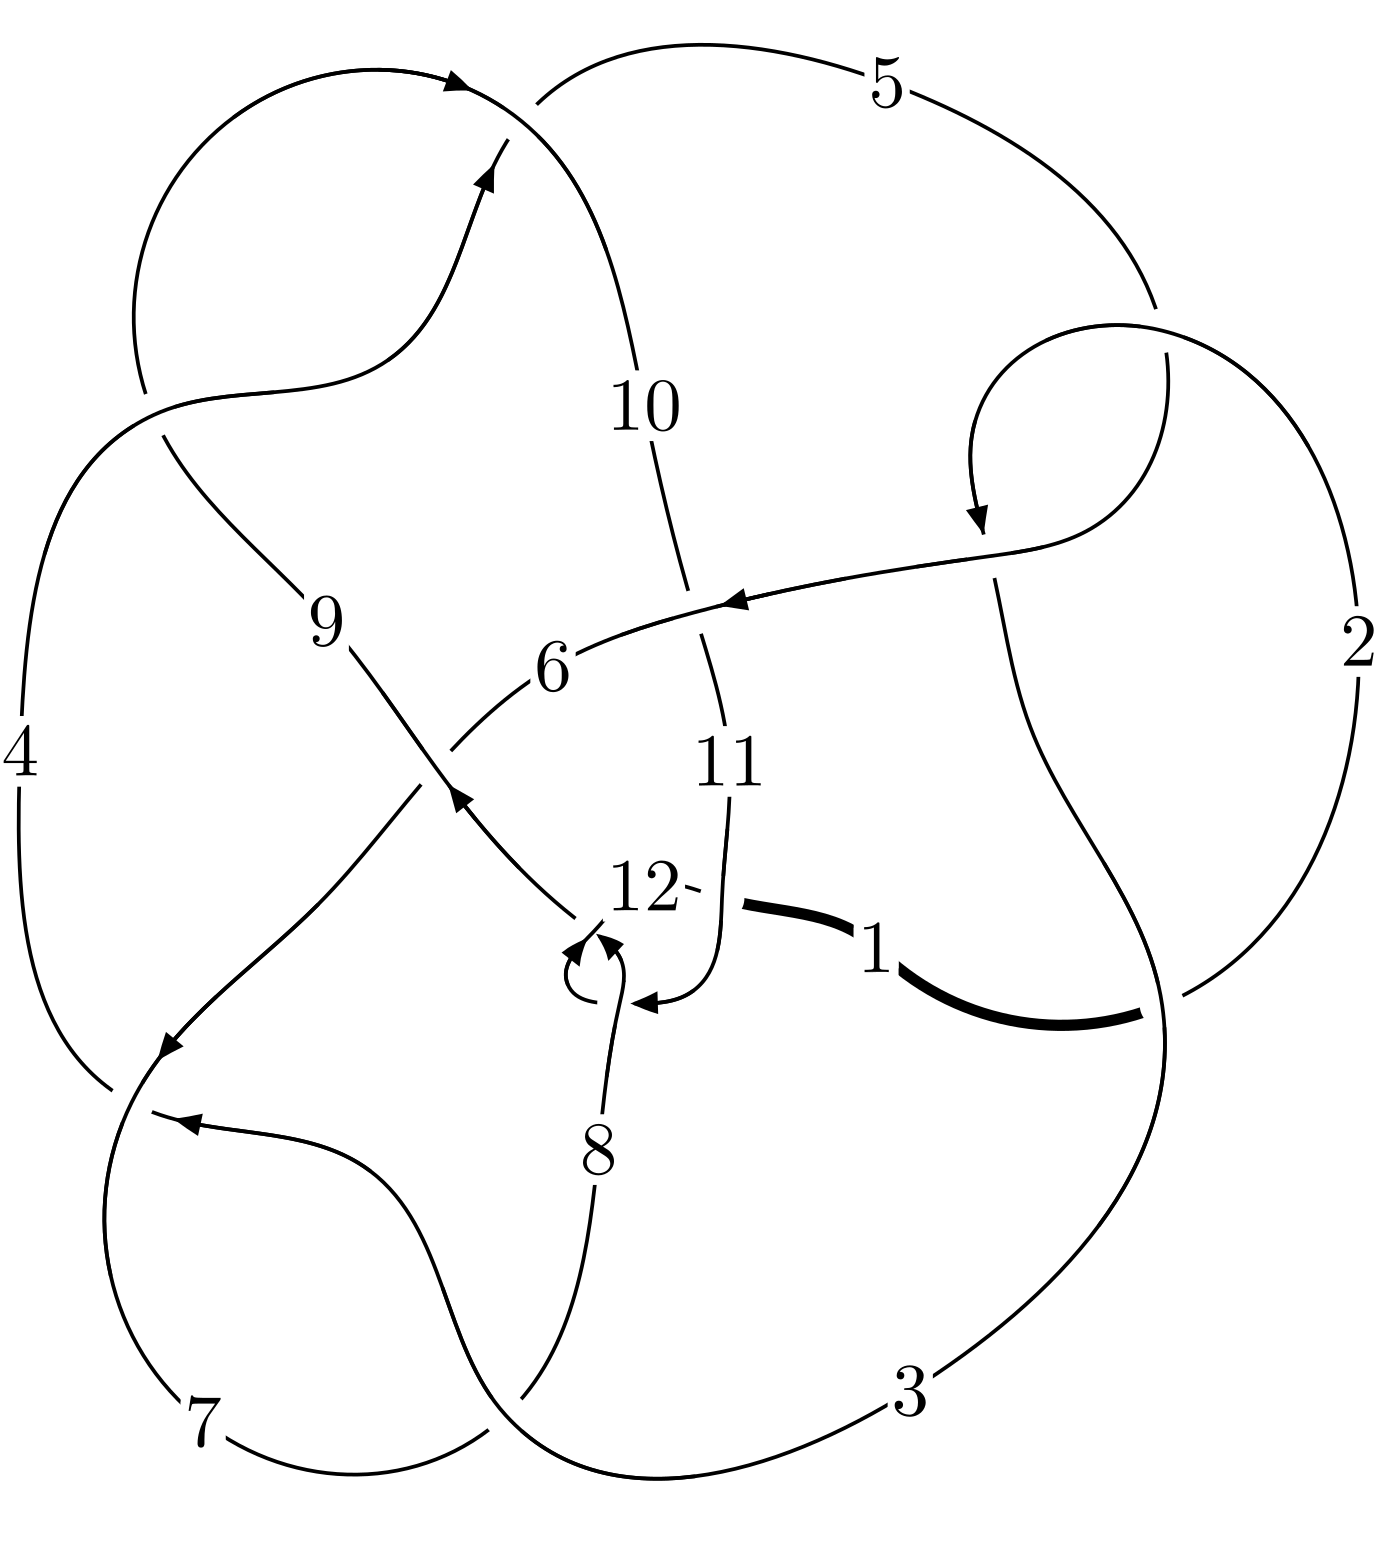
\includegraphics[width=112pt]{../../../GIT/diagram.site/Diagrams/png/2457_12n_0368.png}\\
\ \ \ A knot diagram\footnotemark}&
\allowdisplaybreaks
\textbf{Linearized knot diagam} \\
\cline{2-2}
 &
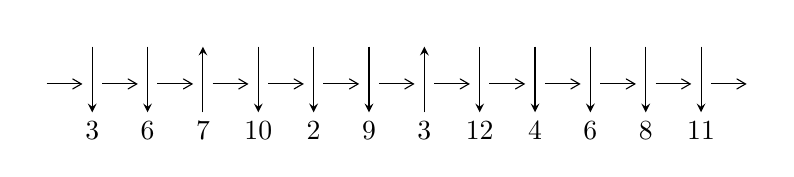
\begin{tikzpicture}[x=20pt, y=17pt]
	% nodes
	\node (C0) at (0, 0) {};
	\node (C1) at (1, 0) {};
	\node (C1U) at (1, +1) {};
	\node (C1D) at (1, -1) {3};

	\node (C2) at (2, 0) {};
	\node (C2U) at (2, +1) {};
	\node (C2D) at (2, -1) {6};

	\node (C3) at (3, 0) {};
	\node (C3U) at (3, +1) {};
	\node (C3D) at (3, -1) {7};

	\node (C4) at (4, 0) {};
	\node (C4U) at (4, +1) {};
	\node (C4D) at (4, -1) {10};

	\node (C5) at (5, 0) {};
	\node (C5U) at (5, +1) {};
	\node (C5D) at (5, -1) {2};

	\node (C6) at (6, 0) {};
	\node (C6U) at (6, +1) {};
	\node (C6D) at (6, -1) {9};

	\node (C7) at (7, 0) {};
	\node (C7U) at (7, +1) {};
	\node (C7D) at (7, -1) {3};

	\node (C8) at (8, 0) {};
	\node (C8U) at (8, +1) {};
	\node (C8D) at (8, -1) {12};

	\node (C9) at (9, 0) {};
	\node (C9U) at (9, +1) {};
	\node (C9D) at (9, -1) {4};

	\node (C10) at (10, 0) {};
	\node (C10U) at (10, +1) {};
	\node (C10D) at (10, -1) {6};

	\node (C11) at (11, 0) {};
	\node (C11U) at (11, +1) {};
	\node (C11D) at (11, -1) {8};

	\node (C12) at (12, 0) {};
	\node (C12U) at (12, +1) {};
	\node (C12D) at (12, -1) {11};
	\node (C13) at (13, 0) {};

	% arrows
	\draw[->,>={angle 60}]
	(C0) edge (C1) (C1) edge (C2) (C2) edge (C3) (C3) edge (C4) (C4) edge (C5) (C5) edge (C6) (C6) edge (C7) (C7) edge (C8) (C8) edge (C9) (C9) edge (C10) (C10) edge (C11) (C11) edge (C12) (C12) edge (C13) ;	\draw[->,>=stealth]
	(C1U) edge (C1D) (C2U) edge (C2D) (C3D) edge (C3U) (C4U) edge (C4D) (C5U) edge (C5D) (C6U) edge (C6D) (C7D) edge (C7U) (C8U) edge (C8D) (C9U) edge (C9D) (C10U) edge (C10D) (C11U) edge (C11D) (C12U) edge (C12D) ;
	\end{tikzpicture} \\
\hhline{~~} \\& 
\textbf{Solving Sequence} \\ \cline{2-2} 
 &
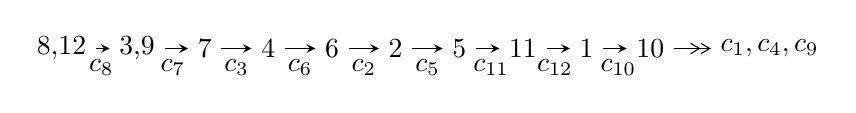
\begin{tikzpicture}[x=23pt, y=7pt]
	% node
	\node (A0) at (-1/8, 0) {8,12};
	\node (A1) at (17/16, 0) {3,9};
	\node (A2) at (17/8, 0) {7};
	\node (A3) at (25/8, 0) {4};
	\node (A4) at (33/8, 0) {6};
	\node (A5) at (41/8, 0) {2};
	\node (A6) at (49/8, 0) {5};
	\node (A7) at (57/8, 0) {11};
	\node (A8) at (65/8, 0) {1};
	\node (A9) at (73/8, 0) {10};
	\node (C1) at (1/2, -1) {$c_{8}$};
	\node (C2) at (13/8, -1) {$c_{7}$};
	\node (C3) at (21/8, -1) {$c_{3}$};
	\node (C4) at (29/8, -1) {$c_{6}$};
	\node (C5) at (37/8, -1) {$c_{2}$};
	\node (C6) at (45/8, -1) {$c_{5}$};
	\node (C7) at (53/8, -1) {$c_{11}$};
	\node (C8) at (61/8, -1) {$c_{12}$};
	\node (C9) at (69/8, -1) {$c_{10}$};
	\node (A10) at (11, 0) {$c_{1},c_{4},c_{9}$};

	% edge
	\draw[->,>=stealth]	
	(A0) edge (A1) (A1) edge (A2) (A2) edge (A3) (A3) edge (A4) (A4) edge (A5) (A5) edge (A6) (A6) edge (A7) (A7) edge (A8) (A8) edge (A9) ;
	\draw[->>,>={angle 60}]	
	(A9) edge (A10);
\end{tikzpicture} \\ 

\end{tabular} \\

\footnotetext{
The image of knot diagram is generated by the software ``\textbf{Draw programme}" developed by Andrew Bartholomew(\url{http://www.layer8.co.uk/maths/draw/index.htm\#Running-draw}), where we modified some parts for our purpose(\url{https://github.com/CATsTAILs/LinksPainter}).
}\phantom \\ \newline 
\centering \textbf{Ideals for irreducible components\footnotemark of $X_{\text{par}}$} 
 
\begin{align*}
I^u_{1}&=\langle 
4.99290\times10^{29} u^{27}-9.04354\times10^{29} u^{26}+\cdots+1.48123\times10^{30} b+2.22464\times10^{30},\\
\phantom{I^u_{1}}&\phantom{= \langle  }1.79527\times10^{31} u^{27}-3.40599\times10^{31} u^{26}+\cdots+4.44370\times10^{30} a+1.93917\times10^{32},\;u^{28}-2 u^{27}+\cdots+15 u-1\rangle \\
I^u_{2}&=\langle 
- u^{15}- u^{14}+\cdots+b-1,\;-6 u^{15}+2 u^{14}+\cdots+a-10,\\
\phantom{I^u_{2}}&\phantom{= \langle  }u^{16}-5 u^{14}+u^{13}+13 u^{12}-3 u^{11}-23 u^{10}+6 u^9+29 u^8-8 u^7-26 u^6+8 u^5+16 u^4-4 u^3-6 u^2+u+1\rangle \\
I^u_{3}&=\langle 
b-1,\;a-1,\;u+1\rangle \\
\\
\end{align*}
\raggedright * 3 irreducible components of $\dim_{\mathbb{C}}=0$, with total 45 representations.\\
\footnotetext{All coefficients of polynomials are rational numbers. But the coefficients are sometimes approximated in decimal forms when there is not enough margin.}
\newpage
\renewcommand{\arraystretch}{1}
\centering \section*{I. $I^u_{1}= \langle 4.99\times10^{29} u^{27}-9.04\times10^{29} u^{26}+\cdots+1.48\times10^{30} b+2.22\times10^{30},\;1.80\times10^{31} u^{27}-3.41\times10^{31} u^{26}+\cdots+4.44\times10^{30} a+1.94\times10^{32},\;u^{28}-2 u^{27}+\cdots+15 u-1 \rangle$}
\flushleft \textbf{(i) Arc colorings}\\
\begin{tabular}{m{7pt} m{180pt} m{7pt} m{180pt} }
\flushright $a_{8}=$&$\begin{pmatrix}1\\0\end{pmatrix}$ \\
\flushright $a_{12}=$&$\begin{pmatrix}0\\u\end{pmatrix}$ \\
\flushright $a_{3}=$&$\begin{pmatrix}-4.04003 u^{27}+7.66476 u^{26}+\cdots+200.372 u-43.6386\\-0.337077 u^{27}+0.610541 u^{26}+\cdots+8.04513 u-1.50188\end{pmatrix}$ \\
\flushright $a_{9}=$&$\begin{pmatrix}1\\u^2\end{pmatrix}$ \\
\flushright $a_{7}=$&$\begin{pmatrix}4.84634 u^{27}-9.14511 u^{26}+\cdots-218.138 u+47.6168\\0.162770 u^{27}-0.345209 u^{26}+\cdots-15.7091 u+2.22482\end{pmatrix}$ \\
\flushright $a_{4}=$&$\begin{pmatrix}-9.48708 u^{27}+18.0943 u^{26}+\cdots+467.082 u-96.8502\\-0.312623 u^{27}+0.470169 u^{26}+\cdots+9.63585 u-2.96138\end{pmatrix}$ \\
\flushright $a_{6}=$&$\begin{pmatrix}4.97301 u^{27}-9.41740 u^{26}+\cdots-230.480 u+49.2941\\0.173164 u^{27}-0.347370 u^{26}+\cdots-15.2980 u+2.20586\end{pmatrix}$ \\
\flushright $a_{2}=$&$\begin{pmatrix}-12.5790 u^{27}+23.8637 u^{26}+\cdots+606.925 u-129.004\\-0.600077 u^{27}+1.10181 u^{26}+\cdots+27.4907 u-4.83602\end{pmatrix}$ \\
\flushright $a_{5}=$&$\begin{pmatrix}-16.7676 u^{27}+31.8085 u^{26}+\cdots+818.466 u-172.294\\-0.699475 u^{27}+1.15355 u^{26}+\cdots+25.6721 u-5.70735\end{pmatrix}$ \\
\flushright $a_{11}=$&$\begin{pmatrix}u\\u\end{pmatrix}$ \\
\flushright $a_{1}=$&$\begin{pmatrix}- u^3\\- u^3+u\end{pmatrix}$ \\
\flushright $a_{10}=$&$\begin{pmatrix}15.6689 u^{27}-29.9384 u^{26}+\cdots-773.348 u+161.864\\0.340769 u^{27}-0.720300 u^{26}+\cdots-15.5800 u+4.83370\end{pmatrix}$\\&\end{tabular}
\flushleft \textbf{(ii) Obstruction class $= -1$}\\~\\
\flushleft \textbf{(iii) Cusp Shapes $= 2.36235 u^{27}-4.45969 u^{26}+\cdots-84.8018 u+5.95686$}\\~\\
\newpage\renewcommand{\arraystretch}{1}
\flushleft \textbf{(iv) u-Polynomials at the component}\newline \\
\begin{tabular}{m{50pt}|m{274pt}}
Crossings & \hspace{64pt}u-Polynomials at each crossing \\
\hline $$\begin{aligned}c_{1}\end{aligned}$$&$\begin{aligned}
&u^{28}+56 u^{27}+\cdots+733262 u+28561
\end{aligned}$\\
\hline $$\begin{aligned}c_{2},c_{5}\end{aligned}$$&$\begin{aligned}
&u^{28}+2 u^{27}+\cdots-1450 u-169
\end{aligned}$\\
\hline $$\begin{aligned}c_{3},c_{7}\end{aligned}$$&$\begin{aligned}
&u^{28}-4 u^{27}+\cdots+156 u+23
\end{aligned}$\\
\hline $$\begin{aligned}c_{4},c_{9}\end{aligned}$$&$\begin{aligned}
&u^{28}-24 u^{26}+\cdots+46 u-43
\end{aligned}$\\
\hline $$\begin{aligned}c_{6}\end{aligned}$$&$\begin{aligned}
&u^{28}-3 u^{27}+\cdots- u-1
\end{aligned}$\\
\hline $$\begin{aligned}c_{8},c_{11}\end{aligned}$$&$\begin{aligned}
&u^{28}+2 u^{27}+\cdots-15 u-1
\end{aligned}$\\
\hline $$\begin{aligned}c_{10}\end{aligned}$$&$\begin{aligned}
&u^{28}-63 u^{26}+\cdots+129664 u+33653
\end{aligned}$\\
\hline $$\begin{aligned}c_{12}\end{aligned}$$&$\begin{aligned}
&u^{28}+26 u^{27}+\cdots+87 u+1
\end{aligned}$\\
\hline
\end{tabular}\\~\\
\newpage\renewcommand{\arraystretch}{1}
\flushleft \textbf{(v) Riley Polynomials at the component}\newline \\
\begin{tabular}{m{50pt}|m{274pt}}
Crossings & \hspace{64pt}Riley Polynomials at each crossing \\
\hline $$\begin{aligned}c_{1}\end{aligned}$$&$\begin{aligned}
&y^{28}-188 y^{27}+\cdots-348035375138 y+815730721
\end{aligned}$\\
\hline $$\begin{aligned}c_{2},c_{5}\end{aligned}$$&$\begin{aligned}
&y^{28}-56 y^{27}+\cdots-733262 y+28561
\end{aligned}$\\
\hline $$\begin{aligned}c_{3},c_{7}\end{aligned}$$&$\begin{aligned}
&y^{28}+32 y^{27}+\cdots+1516 y+529
\end{aligned}$\\
\hline $$\begin{aligned}c_{4},c_{9}\end{aligned}$$&$\begin{aligned}
&y^{28}-48 y^{27}+\cdots-11662 y+1849
\end{aligned}$\\
\hline $$\begin{aligned}c_{6}\end{aligned}$$&$\begin{aligned}
&y^{28}-3 y^{27}+\cdots-13 y+1
\end{aligned}$\\
\hline $$\begin{aligned}c_{8},c_{11}\end{aligned}$$&$\begin{aligned}
&y^{28}-26 y^{27}+\cdots-87 y+1
\end{aligned}$\\
\hline $$\begin{aligned}c_{10}\end{aligned}$$&$\begin{aligned}
&y^{28}-126 y^{27}+\cdots-33547178288 y+1132524409
\end{aligned}$\\
\hline $$\begin{aligned}c_{12}\end{aligned}$$&$\begin{aligned}
&y^{28}-38 y^{27}+\cdots-11231 y+1
\end{aligned}$\\
\hline
\end{tabular}\\~\\
\newpage\flushleft \textbf{(vi) Complex Volumes and Cusp Shapes}
$$\begin{array}{c|c|c}  
\text{Solutions to }I^u_{1}& \I (\text{vol} + \sqrt{-1}CS) & \text{Cusp shape}\\
 \hline 
\begin{aligned}
u &= -0.906896 + 0.646886 I \\
a &= -0.018709 - 0.380835 I \\
b &= -0.638662 + 0.021294 I\end{aligned}
 & \phantom{-}1.71311 + 2.54690 I & -1.43844 - 1.11774 I \\ \hline\begin{aligned}
u &= -0.906896 - 0.646886 I \\
a &= -0.018709 + 0.380835 I \\
b &= -0.638662 - 0.021294 I\end{aligned}
 & \phantom{-}1.71311 - 2.54690 I & -1.43844 + 1.11774 I \\ \hline\begin{aligned}
u &= \phantom{-}0.967377 + 0.607852 I \\
a &= \phantom{-}0.156659 - 0.808047 I \\
b &= \phantom{-}0.094276 - 0.264187 I\end{aligned}
 & -1.84113 - 4.28473 I & -9.39382 + 5.33049 I \\ \hline\begin{aligned}
u &= \phantom{-}0.967377 - 0.607852 I \\
a &= \phantom{-}0.156659 + 0.808047 I \\
b &= \phantom{-}0.094276 + 0.264187 I\end{aligned}
 & -1.84113 + 4.28473 I & -9.39382 - 5.33049 I \\ \hline\begin{aligned}
u &= -1.213110 + 0.327569 I \\
a &= \phantom{-}0.57852 - 1.90768 I \\
b &= -0.26231 - 1.86751 I\end{aligned}
 & -4.18195 + 4.33996 I & -13.7175 - 7.6147 I \\ \hline\begin{aligned}
u &= -1.213110 - 0.327569 I \\
a &= \phantom{-}0.57852 + 1.90768 I \\
b &= -0.26231 + 1.86751 I\end{aligned}
 & -4.18195 - 4.33996 I & -13.7175 + 7.6147 I \\ \hline\begin{aligned}
u &= \phantom{-}0.614251 + 0.338068 I \\
a &= -0.531012 + 0.325089 I \\
b &= \phantom{-}0.489062 - 0.020644 I\end{aligned}
 & -0.982240 + 0.119994 I & -8.17175 + 0.02561 I \\ \hline\begin{aligned}
u &= \phantom{-}0.614251 - 0.338068 I \\
a &= -0.531012 - 0.325089 I \\
b &= \phantom{-}0.489062 + 0.020644 I\end{aligned}
 & -0.982240 - 0.119994 I & -8.17175 - 0.02561 I \\ \hline\begin{aligned}
u &= \phantom{-}0.696063\phantom{ +0.000000I} \\
a &= -0.481673\phantom{ +0.000000I} \\
b &= \phantom{-}0.373251\phantom{ +0.000000I}\end{aligned}
 & -0.946260\phantom{ +0.000000I} & -10.4550\phantom{ +0.000000I} \\ \hline\begin{aligned}
u &= \phantom{-}1.257950 + 0.387635 I \\
a &= -0.74898 - 1.66086 I \\
b &= \phantom{-}0.123685 - 1.210180 I\end{aligned}
 & -4.49564 - 1.87179 I & -14.6317 - 1.5633 I\\
 \hline 
 \end{array}$$\newpage$$\begin{array}{c|c|c}  
\text{Solutions to }I^u_{1}& \I (\text{vol} + \sqrt{-1}CS) & \text{Cusp shape}\\
 \hline 
\begin{aligned}
u &= \phantom{-}1.257950 - 0.387635 I \\
a &= -0.74898 + 1.66086 I \\
b &= \phantom{-}0.123685 + 1.210180 I\end{aligned}
 & -4.49564 + 1.87179 I & -14.6317 + 1.5633 I \\ \hline\begin{aligned}
u &= -0.07059 + 1.45889 I \\
a &= -0.0475163 - 0.0400773 I \\
b &= -0.21400 - 1.78782 I\end{aligned}
 & -18.0323 + 4.3258 I & -11.73246 - 2.08575 I \\ \hline\begin{aligned}
u &= -0.07059 - 1.45889 I \\
a &= -0.0475163 + 0.0400773 I \\
b &= -0.21400 + 1.78782 I\end{aligned}
 & -18.0323 - 4.3258 I & -11.73246 + 2.08575 I \\ \hline\begin{aligned}
u &= \phantom{-}1.50606\phantom{ +0.000000I} \\
a &= -1.25220\phantom{ +0.000000I} \\
b &= -3.31724\phantom{ +0.000000I}\end{aligned}
 & -15.4303\phantom{ +0.000000I} & -22.9460\phantom{ +0.000000I} \\ \hline\begin{aligned}
u &= -0.036535 + 0.484008 I \\
a &= -0.642458 + 0.305211 I \\
b &= -0.141755 + 0.946555 I\end{aligned}
 & -0.78712 - 1.33307 I & -6.90000 + 4.82501 I \\ \hline\begin{aligned}
u &= -0.036535 - 0.484008 I \\
a &= -0.642458 - 0.305211 I \\
b &= -0.141755 - 0.946555 I\end{aligned}
 & -0.78712 + 1.33307 I & -6.90000 - 4.82501 I \\ \hline\begin{aligned}
u &= \phantom{-}1.57314 + 0.15250 I \\
a &= \phantom{-}0.34179 + 1.42667 I \\
b &= -0.20624 + 2.13211 I\end{aligned}
 & -10.36200 + 1.52321 I & -13.77194 - 1.67469 I \\ \hline\begin{aligned}
u &= \phantom{-}1.57314 - 0.15250 I \\
a &= \phantom{-}0.34179 - 1.42667 I \\
b &= -0.20624 - 2.13211 I\end{aligned}
 & -10.36200 - 1.52321 I & -13.77194 + 1.67469 I \\ \hline\begin{aligned}
u &= -1.61185\phantom{ +0.000000I} \\
a &= -0.871275\phantom{ +0.000000I} \\
b &= \phantom{-}0.575915\phantom{ +0.000000I}\end{aligned}
 & -16.6517\phantom{ +0.000000I} & -17.2310\phantom{ +0.000000I} \\ \hline\begin{aligned}
u &= -1.61164 + 0.12556 I \\
a &= -0.01556 + 1.51530 I \\
b &= \phantom{-}0.42383 + 1.60874 I\end{aligned}
 & -11.04510 + 5.13574 I & -13.9862 - 3.3545 I\\
 \hline 
 \end{array}$$\newpage$$\begin{array}{c|c|c}  
\text{Solutions to }I^u_{1}& \I (\text{vol} + \sqrt{-1}CS) & \text{Cusp shape}\\
 \hline 
\begin{aligned}
u &= -1.61164 - 0.12556 I \\
a &= -0.01556 - 1.51530 I \\
b &= \phantom{-}0.42383 - 1.60874 I\end{aligned}
 & -11.04510 - 5.13574 I & -13.9862 + 3.3545 I \\ \hline\begin{aligned}
u &= \phantom{-}0.055371 + 0.305690 I \\
a &= -1.91148 + 0.93139 I \\
b &= \phantom{-}0.441705 - 1.203630 I\end{aligned}
 & -4.59867 - 3.49978 I & -13.2785 + 5.9062 I \\ \hline\begin{aligned}
u &= \phantom{-}0.055371 - 0.305690 I \\
a &= -1.91148 - 0.93139 I \\
b &= \phantom{-}0.441705 + 1.203630 I\end{aligned}
 & -4.59867 + 3.49978 I & -13.2785 - 5.9062 I \\ \hline\begin{aligned}
u &= \phantom{-}1.56528 + 0.69723 I \\
a &= \phantom{-}0.61493 + 1.30760 I \\
b &= -0.73222 + 1.97314 I\end{aligned}
 & \phantom{-}16.4052 - 11.9046 I & -13.05540 + 4.81403 I \\ \hline\begin{aligned}
u &= \phantom{-}1.56528 - 0.69723 I \\
a &= \phantom{-}0.61493 - 1.30760 I \\
b &= -0.73222 - 1.97314 I\end{aligned}
 & \phantom{-}16.4052 + 11.9046 I & -13.05540 - 4.81403 I \\ \hline\begin{aligned}
u &= -1.53853 + 0.79216 I \\
a &= -0.793628 + 0.857092 I \\
b &= \phantom{-}0.34136 + 1.61067 I\end{aligned}
 & \phantom{-}17.0288 + 3.5616 I & -13.06254 + 0. I\phantom{ +0.000000I} \\ \hline\begin{aligned}
u &= -1.53853 - 0.79216 I \\
a &= -0.793628 - 0.857092 I \\
b &= \phantom{-}0.34136 - 1.61067 I\end{aligned}
 & \phantom{-}17.0288 - 3.5616 I & -13.06254 + 0. I\phantom{ +0.000000I} \\ \hline\begin{aligned}
u &= \phantom{-}0.0975704\phantom{ +0.000000I} \\
a &= -30.3600\phantom{ +0.000000I} \\
b &= -1.06939\phantom{ +0.000000I}\end{aligned}
 & -10.1503\phantom{ +0.000000I} & \phantom{-}0.912190\phantom{ +0.000000I}\\
 \hline 
 \end{array}$$\newpage\newpage\renewcommand{\arraystretch}{1}
\centering \section*{II. $I^u_{2}= \langle - u^{15}- u^{14}+\cdots+b-1,\;-6 u^{15}+2 u^{14}+\cdots+a-10,\;u^{16}-5 u^{14}+\cdots+u+1 \rangle$}
\flushleft \textbf{(i) Arc colorings}\\
\begin{tabular}{m{7pt} m{180pt} m{7pt} m{180pt} }
\flushright $a_{8}=$&$\begin{pmatrix}1\\0\end{pmatrix}$ \\
\flushright $a_{12}=$&$\begin{pmatrix}0\\u\end{pmatrix}$ \\
\flushright $a_{3}=$&$\begin{pmatrix}6 u^{15}-2 u^{14}+\cdots-15 u+10\\u^{15}+u^{14}+\cdots-4 u+1\end{pmatrix}$ \\
\flushright $a_{9}=$&$\begin{pmatrix}1\\u^2\end{pmatrix}$ \\
\flushright $a_{7}=$&$\begin{pmatrix}5 u^{15}-4 u^{14}+\cdots-10 u+13\\3 u^{15}-2 u^{14}+\cdots-2 u+3\end{pmatrix}$ \\
\flushright $a_{4}=$&$\begin{pmatrix}13 u^{15}-5 u^{14}+\cdots-30 u+25\\u^{14}- u^{13}+\cdots-5 u+1\end{pmatrix}$ \\
\flushright $a_{6}=$&$\begin{pmatrix}6 u^{15}-4 u^{14}+\cdots-11 u+12\\3 u^{15}-2 u^{14}+\cdots-3 u+3\end{pmatrix}$ \\
\flushright $a_{2}=$&$\begin{pmatrix}16 u^{15}-7 u^{14}+\cdots-35 u+29\\3 u^{15}- u^{14}+\cdots-4 u+5\end{pmatrix}$ \\
\flushright $a_{5}=$&$\begin{pmatrix}-18 u^{15}+9 u^{14}+\cdots+38 u-40\\- u^{15}+5 u^{13}+\cdots+5 u-4\end{pmatrix}$ \\
\flushright $a_{11}=$&$\begin{pmatrix}u\\u\end{pmatrix}$ \\
\flushright $a_{1}=$&$\begin{pmatrix}- u^3\\- u^3+u\end{pmatrix}$ \\
\flushright $a_{10}=$&$\begin{pmatrix}-21 u^{15}+11 u^{14}+\cdots+40 u-40\\-5 u^{15}+3 u^{14}+\cdots+5 u-9\end{pmatrix}$\\&\end{tabular}
\flushleft \textbf{(ii) Obstruction class $= 1$}\\~\\
\flushleft \textbf{(iii) Cusp Shapes $= -13 u^{15}+4 u^{14}+60 u^{13}-31 u^{12}-141 u^{11}+76 u^{10}+230 u^9-132 u^8-260 u^7+157 u^6+200 u^5-136 u^4-96 u^3+62 u^2+25 u-31$}\\~\\
\newpage\renewcommand{\arraystretch}{1}
\flushleft \textbf{(iv) u-Polynomials at the component}\newline \\
\begin{tabular}{m{50pt}|m{274pt}}
Crossings & \hspace{64pt}u-Polynomials at each crossing \\
\hline $$\begin{aligned}c_{1}\end{aligned}$$&$\begin{aligned}
&u^{16}-16 u^{15}+\cdots-8 u+1
\end{aligned}$\\
\hline $$\begin{aligned}c_{2}\end{aligned}$$&$\begin{aligned}
&u^{16}+4 u^{15}+\cdots+4 u+1
\end{aligned}$\\
\hline $$\begin{aligned}c_{3}\end{aligned}$$&$\begin{aligned}
&u^{16}+4 u^{14}+\cdots-6 u+1
\end{aligned}$\\
\hline $$\begin{aligned}c_{4}\end{aligned}$$&$\begin{aligned}
&u^{16}-10 u^{14}+\cdots-2 u-1
\end{aligned}$\\
\hline $$\begin{aligned}c_{5}\end{aligned}$$&$\begin{aligned}
&u^{16}-4 u^{15}+\cdots-4 u+1
\end{aligned}$\\
\hline $$\begin{aligned}c_{6}\end{aligned}$$&$\begin{aligned}
&u^{16}-3 u^{15}+\cdots-3 u-1
\end{aligned}$\\
\hline $$\begin{aligned}c_{7}\end{aligned}$$&$\begin{aligned}
&u^{16}+4 u^{14}+\cdots+6 u+1
\end{aligned}$\\
\hline $$\begin{aligned}c_{8}\end{aligned}$$&$\begin{aligned}
&u^{16}-5 u^{14}+\cdots+u+1
\end{aligned}$\\
\hline $$\begin{aligned}c_{9}\end{aligned}$$&$\begin{aligned}
&u^{16}-10 u^{14}+\cdots+2 u-1
\end{aligned}$\\
\hline $$\begin{aligned}c_{10}\end{aligned}$$&$\begin{aligned}
&u^{16}+2 u^{15}+\cdots+7 u^2-1
\end{aligned}$\\
\hline $$\begin{aligned}c_{11}\end{aligned}$$&$\begin{aligned}
&u^{16}-5 u^{14}+\cdots- u+1
\end{aligned}$\\
\hline $$\begin{aligned}c_{12}\end{aligned}$$&$\begin{aligned}
&u^{16}+10 u^{15}+\cdots+13 u+1
\end{aligned}$\\
\hline
\end{tabular}\\~\\
\newpage\renewcommand{\arraystretch}{1}
\flushleft \textbf{(v) Riley Polynomials at the component}\newline \\
\begin{tabular}{m{50pt}|m{274pt}}
Crossings & \hspace{64pt}Riley Polynomials at each crossing \\
\hline $$\begin{aligned}c_{1}\end{aligned}$$&$\begin{aligned}
&y^{16}-52 y^{15}+\cdots+20 y+1
\end{aligned}$\\
\hline $$\begin{aligned}c_{2},c_{5}\end{aligned}$$&$\begin{aligned}
&y^{16}-16 y^{15}+\cdots-8 y+1
\end{aligned}$\\
\hline $$\begin{aligned}c_{3},c_{7}\end{aligned}$$&$\begin{aligned}
&y^{16}+8 y^{15}+\cdots-10 y+1
\end{aligned}$\\
\hline $$\begin{aligned}c_{4},c_{9}\end{aligned}$$&$\begin{aligned}
&y^{16}-20 y^{15}+\cdots+4 y+1
\end{aligned}$\\
\hline $$\begin{aligned}c_{6}\end{aligned}$$&$\begin{aligned}
&y^{16}+y^{15}+\cdots-15 y+1
\end{aligned}$\\
\hline $$\begin{aligned}c_{8},c_{11}\end{aligned}$$&$\begin{aligned}
&y^{16}-10 y^{15}+\cdots-13 y+1
\end{aligned}$\\
\hline $$\begin{aligned}c_{10}\end{aligned}$$&$\begin{aligned}
&y^{16}-38 y^{15}+\cdots-14 y+1
\end{aligned}$\\
\hline $$\begin{aligned}c_{12}\end{aligned}$$&$\begin{aligned}
&y^{16}+2 y^{15}+\cdots-17 y+1
\end{aligned}$\\
\hline
\end{tabular}\\~\\
\newpage\flushleft \textbf{(vi) Complex Volumes and Cusp Shapes}
$$\begin{array}{c|c|c}  
\text{Solutions to }I^u_{2}& \I (\text{vol} + \sqrt{-1}CS) & \text{Cusp shape}\\
 \hline 
\begin{aligned}
u &= \phantom{-}0.772761 + 0.712653 I \\
a &= \phantom{-}0.214642 + 0.139490 I \\
b &= -0.174212 + 0.983327 I\end{aligned}
 & -3.18731 - 4.89171 I & -13.3342 + 7.1832 I \\ \hline\begin{aligned}
u &= \phantom{-}0.772761 - 0.712653 I \\
a &= \phantom{-}0.214642 - 0.139490 I \\
b &= -0.174212 - 0.983327 I\end{aligned}
 & -3.18731 + 4.89171 I & -13.3342 - 7.1832 I \\ \hline\begin{aligned}
u &= -1.026470 + 0.385848 I \\
a &= \phantom{-}0.97974 - 2.34875 I \\
b &= -0.64749 - 1.56601 I\end{aligned}
 & -6.20371 + 5.58512 I & -14.9139 - 6.6172 I \\ \hline\begin{aligned}
u &= -1.026470 - 0.385848 I \\
a &= \phantom{-}0.97974 + 2.34875 I \\
b &= -0.64749 + 1.56601 I\end{aligned}
 & -6.20371 - 5.58512 I & -14.9139 + 6.6172 I \\ \hline\begin{aligned}
u &= -0.868992 + 0.775777 I \\
a &= \phantom{-}0.422206 - 0.337071 I \\
b &= -0.267354 + 0.100433 I\end{aligned}
 & \phantom{-}1.11054 + 2.92387 I & -11.66623 - 5.71389 I \\ \hline\begin{aligned}
u &= -0.868992 - 0.775777 I \\
a &= \phantom{-}0.422206 + 0.337071 I \\
b &= -0.267354 - 0.100433 I\end{aligned}
 & \phantom{-}1.11054 - 2.92387 I & -11.66623 + 5.71389 I \\ \hline\begin{aligned}
u &= \phantom{-}1.153510 + 0.323030 I \\
a &= -0.52474 - 1.80473 I \\
b &= -0.125626 - 1.307330 I\end{aligned}
 & -4.07711 - 3.14561 I & -13.9405 + 2.6304 I \\ \hline\begin{aligned}
u &= \phantom{-}1.153510 - 0.323030 I \\
a &= -0.52474 + 1.80473 I \\
b &= -0.125626 + 1.307330 I\end{aligned}
 & -4.07711 + 3.14561 I & -13.9405 - 2.6304 I \\ \hline\begin{aligned}
u &= -0.730829 + 0.328251 I \\
a &= -0.476380 - 0.106565 I \\
b &= -0.722249 + 1.146800 I\end{aligned}
 & -5.07627 - 2.52540 I & -16.3893 + 0.5079 I \\ \hline\begin{aligned}
u &= -0.730829 - 0.328251 I \\
a &= -0.476380 + 0.106565 I \\
b &= -0.722249 - 1.146800 I\end{aligned}
 & -5.07627 + 2.52540 I & -16.3893 - 0.5079 I\\
 \hline 
 \end{array}$$\newpage$$\begin{array}{c|c|c}  
\text{Solutions to }I^u_{2}& \I (\text{vol} + \sqrt{-1}CS) & \text{Cusp shape}\\
 \hline 
\begin{aligned}
u &= \phantom{-}1.004110 + 0.721375 I \\
a &= -1.101500 - 0.625779 I \\
b &= \phantom{-}0.144368 - 1.128410 I\end{aligned}
 & -3.89724 - 0.61018 I & -12.26838 + 0.63265 I \\ \hline\begin{aligned}
u &= \phantom{-}1.004110 - 0.721375 I \\
a &= -1.101500 + 0.625779 I \\
b &= \phantom{-}0.144368 + 1.128410 I\end{aligned}
 & -3.89724 + 0.61018 I & -12.26838 - 0.63265 I \\ \hline\begin{aligned}
u &= \phantom{-}0.698430 + 0.203647 I \\
a &= -1.272980 + 0.463255 I \\
b &= \phantom{-}0.148546 + 0.648408 I\end{aligned}
 & -2.24714 + 0.87508 I & -15.0335 - 1.9463 I \\ \hline\begin{aligned}
u &= \phantom{-}0.698430 - 0.203647 I \\
a &= -1.272980 - 0.463255 I \\
b &= \phantom{-}0.148546 - 0.648408 I\end{aligned}
 & -2.24714 - 0.87508 I & -15.0335 + 1.9463 I \\ \hline\begin{aligned}
u &= -0.491820\phantom{ +0.000000I} \\
a &= \phantom{-}7.05656\phantom{ +0.000000I} \\
b &= \phantom{-}1.05815\phantom{ +0.000000I}\end{aligned}
 & -10.4382\phantom{ +0.000000I} & -27.2890\phantom{ +0.000000I} \\ \hline\begin{aligned}
u &= -1.51322\phantom{ +0.000000I} \\
a &= \phantom{-}0.461470\phantom{ +0.000000I} \\
b &= \phantom{-}2.22988\phantom{ +0.000000I}\end{aligned}
 & -14.7824\phantom{ +0.000000I} & -9.61910\phantom{ +0.000000I}\\
 \hline 
 \end{array}$$\newpage\newpage\renewcommand{\arraystretch}{1}
\centering \section*{III. $I^u_{3}= \langle b-1,\;a-1,\;u+1 \rangle$}
\flushleft \textbf{(i) Arc colorings}\\
\begin{tabular}{m{7pt} m{180pt} m{7pt} m{180pt} }
\flushright $a_{8}=$&$\begin{pmatrix}1\\0\end{pmatrix}$ \\
\flushright $a_{12}=$&$\begin{pmatrix}0\\-1\end{pmatrix}$ \\
\flushright $a_{3}=$&$\begin{pmatrix}1\\1\end{pmatrix}$ \\
\flushright $a_{9}=$&$\begin{pmatrix}1\\1\end{pmatrix}$ \\
\flushright $a_{7}=$&$\begin{pmatrix}2\\1\end{pmatrix}$ \\
\flushright $a_{4}=$&$\begin{pmatrix}3\\2\end{pmatrix}$ \\
\flushright $a_{6}=$&$\begin{pmatrix}1\\0\end{pmatrix}$ \\
\flushright $a_{2}=$&$\begin{pmatrix}2\\1\end{pmatrix}$ \\
\flushright $a_{5}=$&$\begin{pmatrix}-1\\-1\end{pmatrix}$ \\
\flushright $a_{11}=$&$\begin{pmatrix}-1\\-1\end{pmatrix}$ \\
\flushright $a_{1}=$&$\begin{pmatrix}1\\0\end{pmatrix}$ \\
\flushright $a_{10}=$&$\begin{pmatrix}-2\\-1\end{pmatrix}$\\&\end{tabular}
\flushleft \textbf{(ii) Obstruction class $= -1$}\\~\\
\flushleft \textbf{(iii) Cusp Shapes $= -18$}\\~\\
\newpage\renewcommand{\arraystretch}{1}
\flushleft \textbf{(iv) u-Polynomials at the component}\newline \\
\begin{tabular}{m{50pt}|m{274pt}}
Crossings & \hspace{64pt}u-Polynomials at each crossing \\
\hline $$\begin{aligned}c_{1},c_{2},c_{3}\\c_{5},c_{6},c_{7}\\c_{12}\end{aligned}$$&$\begin{aligned}
&u+1
\end{aligned}$\\
\hline $$\begin{aligned}c_{4},c_{8},c_{9}\\c_{10},c_{11}\end{aligned}$$&$\begin{aligned}
&u-1
\end{aligned}$\\
\hline
\end{tabular}\\~\\
\newpage\renewcommand{\arraystretch}{1}
\flushleft \textbf{(v) Riley Polynomials at the component}\newline \\
\begin{tabular}{m{50pt}|m{274pt}}
Crossings & \hspace{64pt}Riley Polynomials at each crossing \\
\hline $$\begin{aligned}c_{1},c_{2},c_{3}\\c_{4},c_{5},c_{6}\\c_{7},c_{8},c_{9}\\c_{10},c_{11},c_{12}\end{aligned}$$&$\begin{aligned}
&y-1
\end{aligned}$\\
\hline
\end{tabular}\\~\\
\newpage\flushleft \textbf{(vi) Complex Volumes and Cusp Shapes}
$$\begin{array}{c|c|c}  
\text{Solutions to }I^u_{3}& \I (\text{vol} + \sqrt{-1}CS) & \text{Cusp shape}\\
 \hline 
\begin{aligned}
u &= -1.00000\phantom{ +0.000000I} \\
a &= \phantom{-}1.00000\phantom{ +0.000000I} \\
b &= \phantom{-}1.00000\phantom{ +0.000000I}\end{aligned}
 & -4.93480\phantom{ +0.000000I} & -18.0000\phantom{ +0.000000I}\\
 \hline 
 \end{array}$$\newpage
\newpage\renewcommand{\arraystretch}{1}
\centering \section*{ IV. u-Polynomials}
\begin{tabular}{m{50pt}|m{274pt}}
Crossings & \hspace{64pt}u-Polynomials at each crossing \\
\hline $$\begin{aligned}c_{1}\end{aligned}$$&$\begin{aligned}
&(u+1)(u^{16}-16 u^{15}+\cdots-8 u+1)\\
&\cdot(u^{28}+56 u^{27}+\cdots+733262 u+28561)
\end{aligned}$\\
\hline $$\begin{aligned}c_{2}\end{aligned}$$&$\begin{aligned}
&(u+1)(u^{16}+4 u^{15}+\cdots+4 u+1)(u^{28}+2 u^{27}+\cdots-1450 u-169)
\end{aligned}$\\
\hline $$\begin{aligned}c_{3}\end{aligned}$$&$\begin{aligned}
&(u+1)(u^{16}+4 u^{14}+\cdots-6 u+1)(u^{28}-4 u^{27}+\cdots+156 u+23)
\end{aligned}$\\
\hline $$\begin{aligned}c_{4}\end{aligned}$$&$\begin{aligned}
&(u-1)(u^{16}-10 u^{14}+\cdots-2 u-1)(u^{28}-24 u^{26}+\cdots+46 u-43)
\end{aligned}$\\
\hline $$\begin{aligned}c_{5}\end{aligned}$$&$\begin{aligned}
&(u+1)(u^{16}-4 u^{15}+\cdots-4 u+1)(u^{28}+2 u^{27}+\cdots-1450 u-169)
\end{aligned}$\\
\hline $$\begin{aligned}c_{6}\end{aligned}$$&$\begin{aligned}
&(u+1)(u^{16}-3 u^{15}+\cdots-3 u-1)(u^{28}-3 u^{27}+\cdots- u-1)
\end{aligned}$\\
\hline $$\begin{aligned}c_{7}\end{aligned}$$&$\begin{aligned}
&(u+1)(u^{16}+4 u^{14}+\cdots+6 u+1)(u^{28}-4 u^{27}+\cdots+156 u+23)
\end{aligned}$\\
\hline $$\begin{aligned}c_{8}\end{aligned}$$&$\begin{aligned}
&(u-1)(u^{16}-5 u^{14}+\cdots+u+1)(u^{28}+2 u^{27}+\cdots-15 u-1)
\end{aligned}$\\
\hline $$\begin{aligned}c_{9}\end{aligned}$$&$\begin{aligned}
&(u-1)(u^{16}-10 u^{14}+\cdots+2 u-1)(u^{28}-24 u^{26}+\cdots+46 u-43)
\end{aligned}$\\
\hline $$\begin{aligned}c_{10}\end{aligned}$$&$\begin{aligned}
&(u-1)(u^{16}+2 u^{15}+\cdots+7 u^2-1)\\
&\cdot(u^{28}-63 u^{26}+\cdots+129664 u+33653)
\end{aligned}$\\
\hline $$\begin{aligned}c_{11}\end{aligned}$$&$\begin{aligned}
&(u-1)(u^{16}-5 u^{14}+\cdots- u+1)(u^{28}+2 u^{27}+\cdots-15 u-1)
\end{aligned}$\\
\hline $$\begin{aligned}c_{12}\end{aligned}$$&$\begin{aligned}
&(u+1)(u^{16}+10 u^{15}+\cdots+13 u+1)(u^{28}+26 u^{27}+\cdots+87 u+1)
\end{aligned}$\\
\hline
\end{tabular}\newpage\renewcommand{\arraystretch}{1}
\centering \section*{ V. Riley Polynomials}
\begin{tabular}{m{50pt}|m{274pt}}
Crossings & \hspace{64pt}Riley Polynomials at each crossing \\
\hline $$\begin{aligned}c_{1}\end{aligned}$$&$\begin{aligned}
&(y-1)(y^{16}-52 y^{15}+\cdots+20 y+1)\\
&\cdot(y^{28}-188 y^{27}+\cdots-348035375138 y+815730721)
\end{aligned}$\\
\hline $$\begin{aligned}c_{2},c_{5}\end{aligned}$$&$\begin{aligned}
&(y-1)(y^{16}-16 y^{15}+\cdots-8 y+1)\\
&\cdot(y^{28}-56 y^{27}+\cdots-733262 y+28561)
\end{aligned}$\\
\hline $$\begin{aligned}c_{3},c_{7}\end{aligned}$$&$\begin{aligned}
&(y-1)(y^{16}+8 y^{15}+\cdots-10 y+1)(y^{28}+32 y^{27}+\cdots+1516 y+529)
\end{aligned}$\\
\hline $$\begin{aligned}c_{4},c_{9}\end{aligned}$$&$\begin{aligned}
&(y-1)(y^{16}-20 y^{15}+\cdots+4 y+1)(y^{28}-48 y^{27}+\cdots-11662 y+1849)
\end{aligned}$\\
\hline $$\begin{aligned}c_{6}\end{aligned}$$&$\begin{aligned}
&(y-1)(y^{16}+y^{15}+\cdots-15 y+1)(y^{28}-3 y^{27}+\cdots-13 y+1)
\end{aligned}$\\
\hline $$\begin{aligned}c_{8},c_{11}\end{aligned}$$&$\begin{aligned}
&(y-1)(y^{16}-10 y^{15}+\cdots-13 y+1)(y^{28}-26 y^{27}+\cdots-87 y+1)
\end{aligned}$\\
\hline $$\begin{aligned}c_{10}\end{aligned}$$&$\begin{aligned}
&(y-1)(y^{16}-38 y^{15}+\cdots-14 y+1)\\
&\cdot(y^{28}-126 y^{27}+\cdots-33547178288 y+1132524409)
\end{aligned}$\\
\hline $$\begin{aligned}c_{12}\end{aligned}$$&$\begin{aligned}
&(y-1)(y^{16}+2 y^{15}+\cdots-17 y+1)(y^{28}-38 y^{27}+\cdots-11231 y+1)
\end{aligned}$\\
\hline
\end{tabular}
\vskip 2pc
\end{document}